\documentclass[conference]{IEEEtran}
\usepackage[cmex10]{amsmath}
\usepackage{xcolor}
\usepackage{graphicx}
\hyphenation{op-tical net-works semi-conduc-tor}

\begin{document}
\title{LNA Design\\ECE 432 Microwave Circuit Design II}
\author{\IEEEauthorblockN{Jackson Pugh}
\IEEEauthorblockN{Michael Woodruff}
\IEEEauthorblockA{Portland State University\\
Portland, OR 97207}}
\maketitle
\IEEEpeerreviewmaketitle

\begin{abstract}
This report documents the design, simulation, and testing of a 10dB Low Noise Aplifier (LNA) suitable for opperation between 2.4GHz and 2.6GHz using the SAV-541+ E-PHEMT transistor. The design was completed and simulated in Agilent's Advanced Design System software. Good results were acheived in simulation over the required frequency range. However, when constructed and tested, the amplifier was determined to unstably oscillate instead of amplifying. Possible reasons for this are discussed.
 \end{abstract}

\section{Intrduction}
Low Noise Amplifiers are useful when attempting to amplify a signal that is very close to the noise floor, such as a broadcast signal. The particular application for the amplifier descussed in this report was an FSK reciever using 2.4GHz and 2.6GHz signals. The LNA was to be connected to an impedance matching network and antenna on the input side. The output was to drive a frequency detector that determine which of the two frequencies was being recieved. Both of these circuits are beyond the scope of this report but serve to frame the context in which the LNA was designed for. LNA characteristics that of primary concern when designing for such an application are the gain, noise figure, and return loss. These are generally specified for an LNA prior to design as they have the most significant impact on performance. Other design constraints considered for this LNA were supply voltage and maximum power consumption.

\section{LNA Design}
The LNA design is comprised of Minicircuit's low noise SAV-541+ transistor.  Consideration of a suitable bias network is required for gain and stability.  Looking at the SAV-541+ datasheet\cite{sav541datasheet}, a good place to bias the transistor is $I_{DS}$ = 60 mA at $V_{DS}$ = 3 V.  The recommended application circuit provided in the datasheet is used in the design.   The BJT current mirror helps draw $I_{DS}$ to 60 mA.  The supply power was chosen to be 3.7 V (instead of 3.3 V) due to the 0.7 V drop from the BJT current mirror.

\begin{table}[!b]
\caption{LNA Design Constraints}
\centering
    \begin{tabular}{c c c}
    
  	Frequency & 2.4 to 2.6 & (GHz)\\
	Gain (min) & 10 & (dB)\\
	Noise Figure (max) & 2.5 & (dB)\\
	Input Return Loss (min) & 10 & (dB)\\
	Output return Loss (min) & 10 & (dB)\\
	Supply Voltage & 3.3 & (V)\\
	Supply Current (max) & 100 & (mA)\\
    \end{tabular}
\label{tab:fsk24}
\end{table}

Figure~\ref{fig:dccircuit} shows the bias network for the transistor circuit.  Figure~\ref{fig:dcvalues} shows the DC measurements of the parameters of interest.  Figure~\ref{fig:sparamresult} shows the S-Parameter comparison between the bias network circuit and the manufacturer S2P data.  The bias network shows little discrepency but works as expected.

\begin{figure}[!h]
\centering
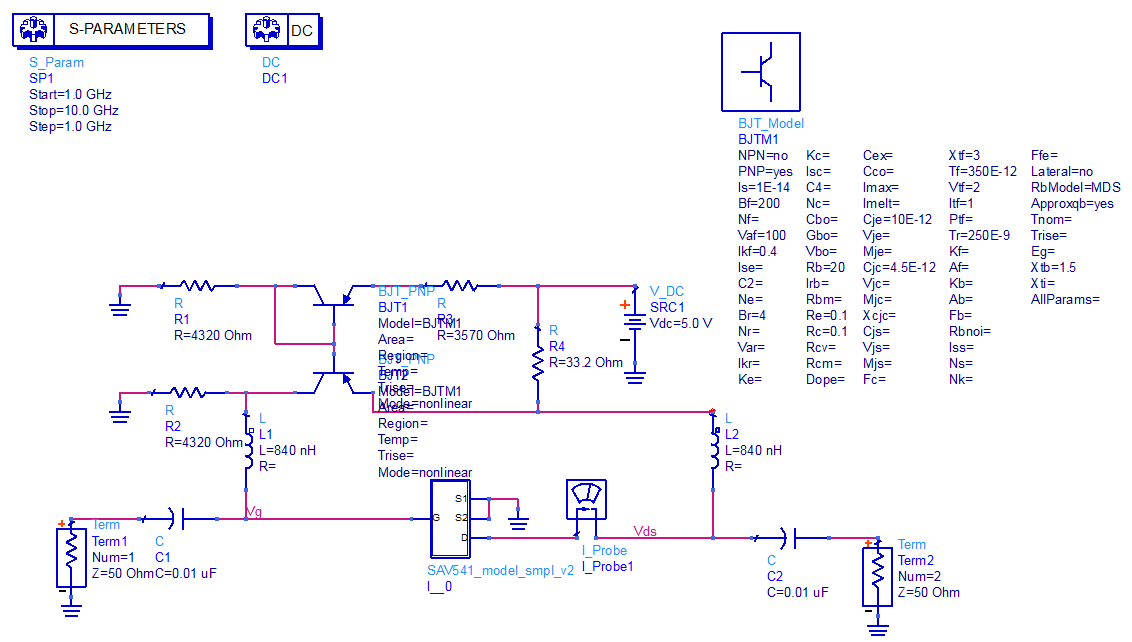
\includegraphics[width=2.5in]{pics/DCBiasNetwork.png}
\caption{DC bias network for the SAV-541+ transistor.}
\label{fig:dccircuit}
\end{figure}

\begin{figure}[!h]
\centering
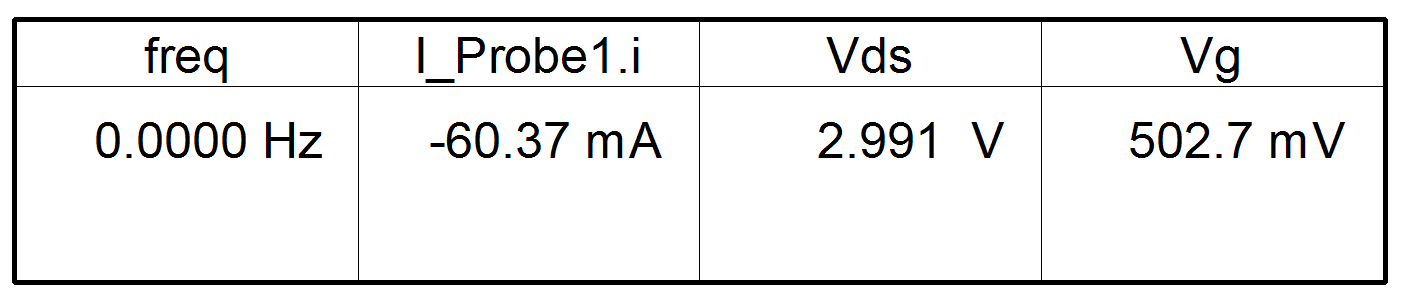
\includegraphics[width=2.5in]{pics/DCBiasResults.png}
\caption{Current and voltage  parameters from the DC bias network for the SAV-541+ transistor.}
\label{fig:dcvalues}
\end{figure}

\begin{figure}[!h]
\centering
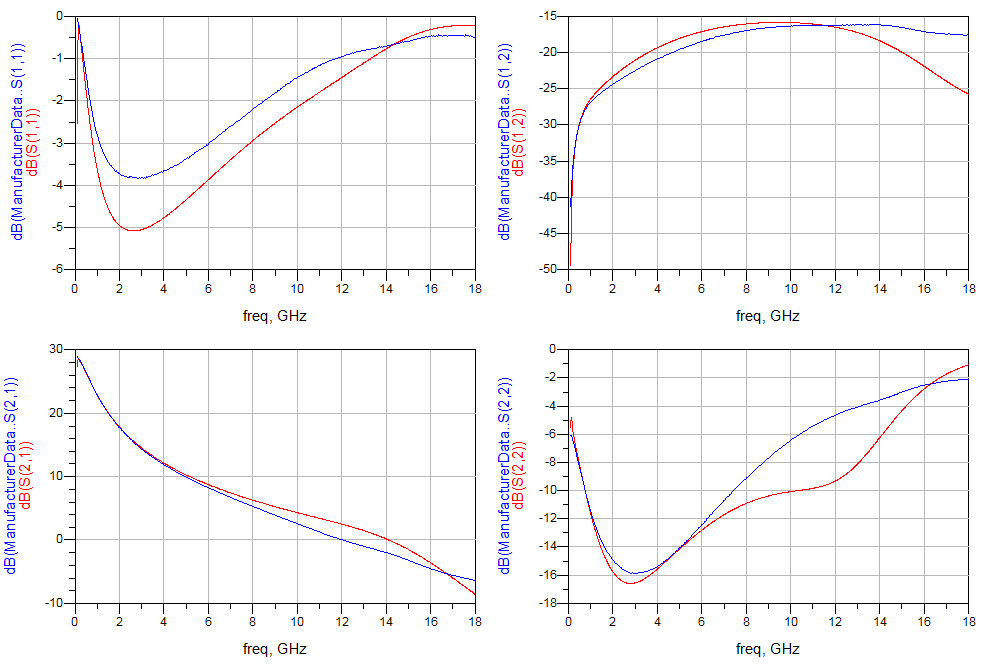
\includegraphics[width=2.5in]{pics/SParameterComparison.png}
\caption{S-Parameter simulation result comparison between the bias network and the manufacturer S2P data file.}
\label{fig:sparamresult}
\end{figure}

Figure~\ref{fig:designguide} shows various information provided by the ADS amplifier design guide tool.  Observing the Stability Factor, K ($mu_{source}$/$mu_{load}$) graph, the circuit is potentially unstable below around 4 GHz.  Thus, stabilizing resistors will be necessary in order to make the transistor unconditionally stable between 2.4 - 2.6 GHz (the intended frequency range).

\begin{figure}[!h]
\centering
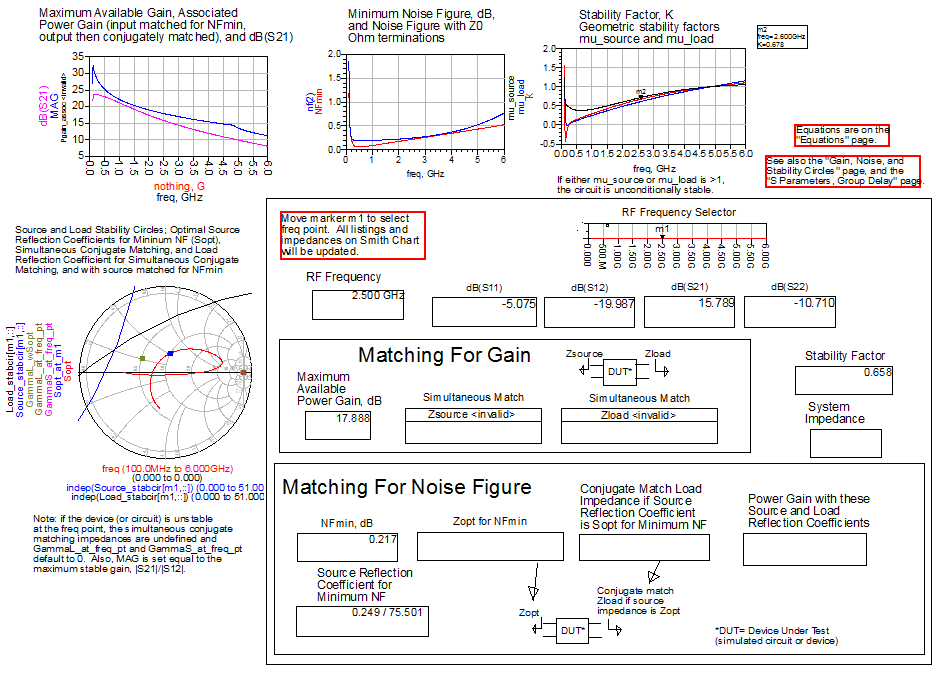
\includegraphics[width=2.5in]{pics/DesignGuideUnoptimized.png}
\caption{Amplifier design guide generated in ADS for the bias network for the SAV-541+ transistor.}
\label{fig:designguide}
\end{figure}

Figure~\ref{fig:designcuidecircuitstabilized} shows added feedback to the transistor used to stablize it unconditionally (under 3 GHz).  After tweaking the circuit for stability, Figure~\ref{fig:designcuidesimulationstabilized} shows the Design Guide for the stabilzed circuit. It shows the circuit is unconditionally stable with a gain of 12.225 dB.

\begin{figure}[!h]
\centering
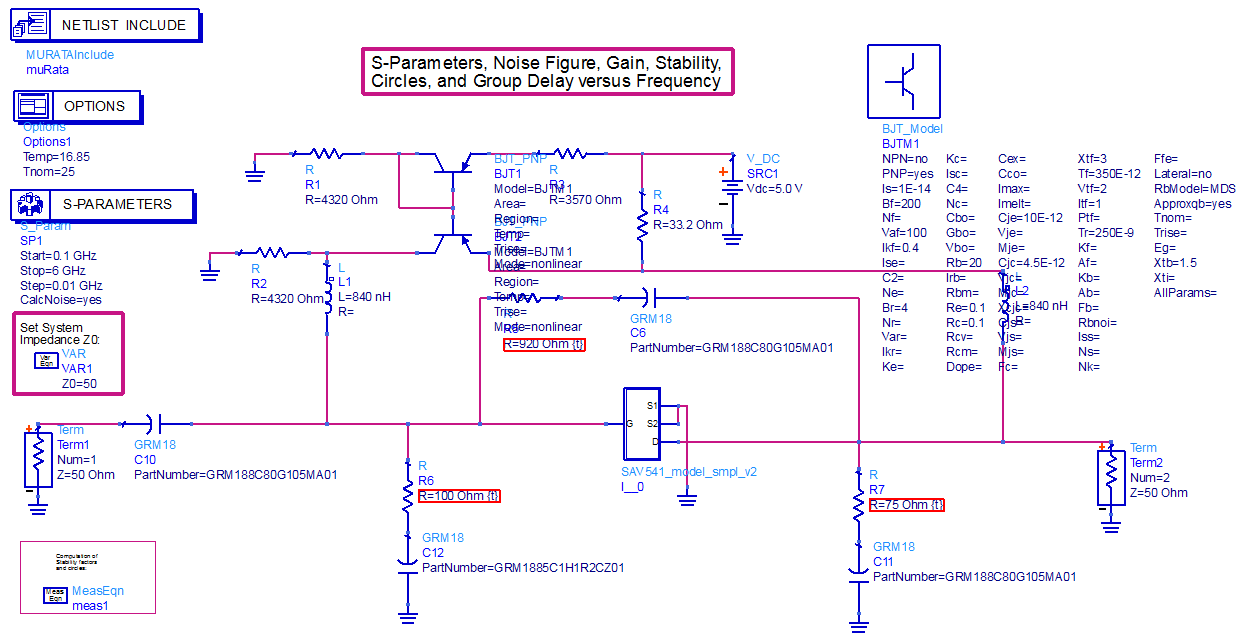
\includegraphics[width=2.5in]{pics/DesignGuideStablizedCircuit.png}
\caption{Stabilized transistor bias circuit for the SAV-541+ using feedback and stabilizing resistors.}
\label{fig:designcuidecircuitstabilized}
\end{figure}

\begin{figure}[!h]
\centering
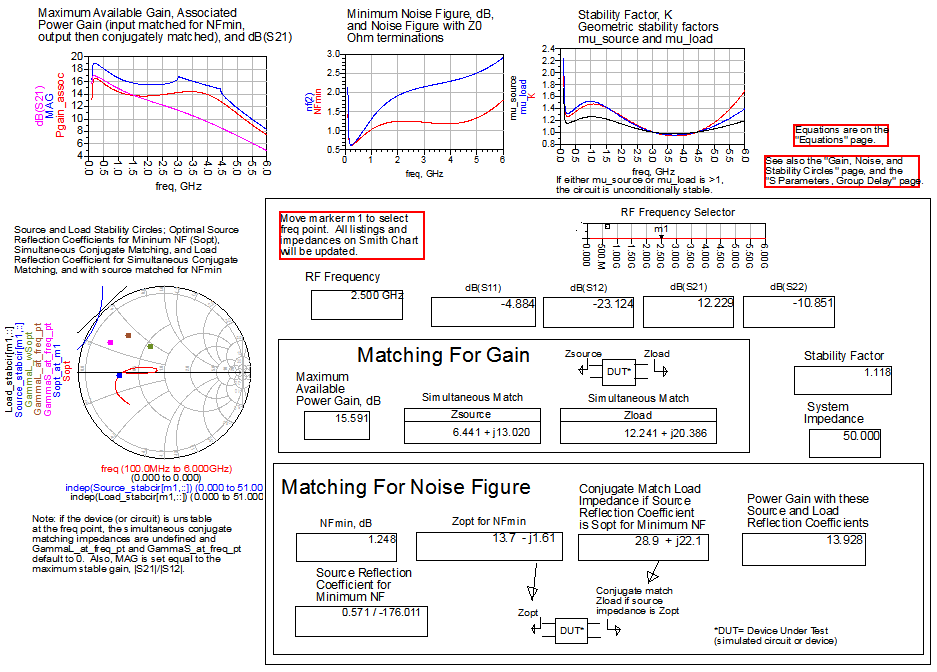
\includegraphics[width=2.5in]{pics/DesignGuideStablizedSimulation.png}
\caption{Amplifier design guide generated in ADS for the bias network for the SAV-541+ transistor.}
\label{fig:designcuidesimulationstabilized}
\end{figure}

The circuit now needs transmission line in order to be able to manufacture the board.  As expected, adding transmission line to the circuit caused the transistor to become potentially unstable.  Thus, it was required to tune the feedback components again.  Figure~\ref{fig:finalstabcircuit} shows the finalized stabilizing circuit for the SAV-541+ transistor.  Figure~\ref{fig:finalstabsimulation} shows the design guide plots.  By observing the $mu_{load}$/$mu_{source}$, the circuit will be unconditionally stable between 0.1 GHz - 6 GHz.  In addition, the gain is above 10 dB.

\begin{figure}[!h]
\centering
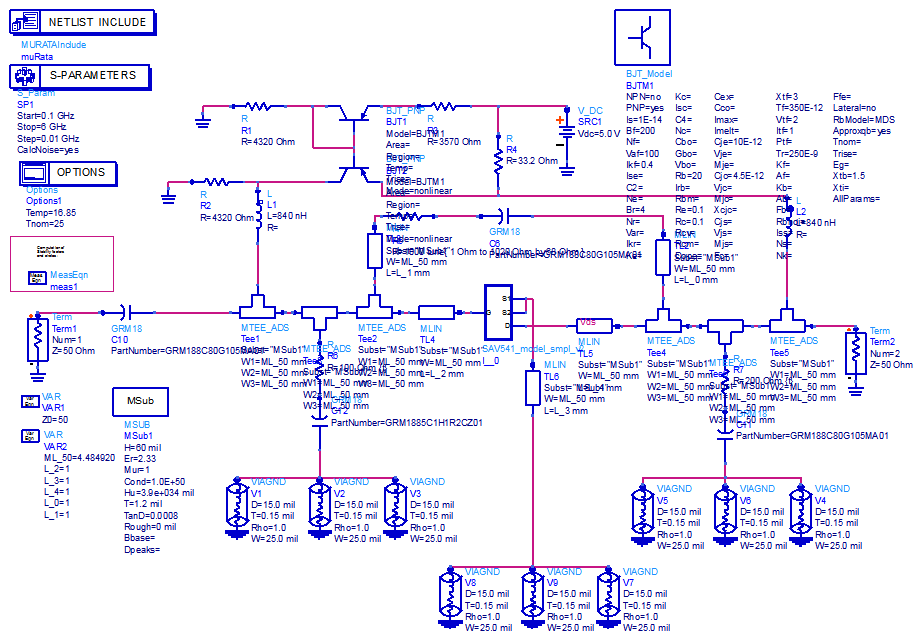
\includegraphics[width=2.5in]{pics/FinalStabilizingCircuit.png}
\caption{Final stabilizing circuit for the SAV-541+ transistor.}
\label{fig:finalstabcircuit}
\end{figure}

\begin{figure}[!h]
\centering
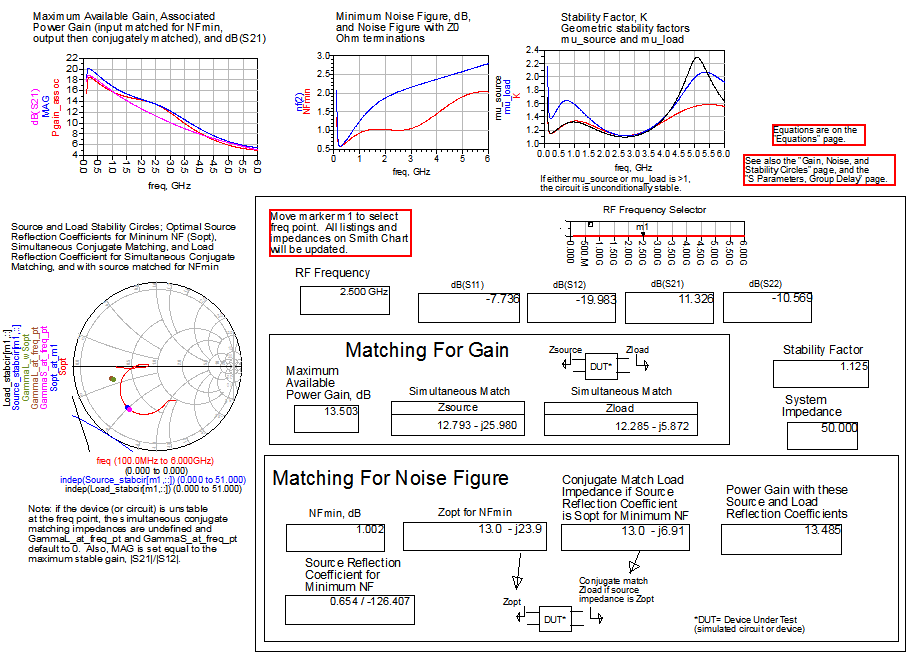
\includegraphics[width=2.5in]{pics/FinalStabilizingSimulation.png}
\caption{ADS design guide simulation results for the stabilizing circuit for the SAV-541+ transistor.}
\label{fig:finalstabsimulation}
\end{figure}

Figure~\ref{fig:lnaLayout} shows the layout which will be used to manufacture the physical board.
\begin{figure}[!h]
\centering
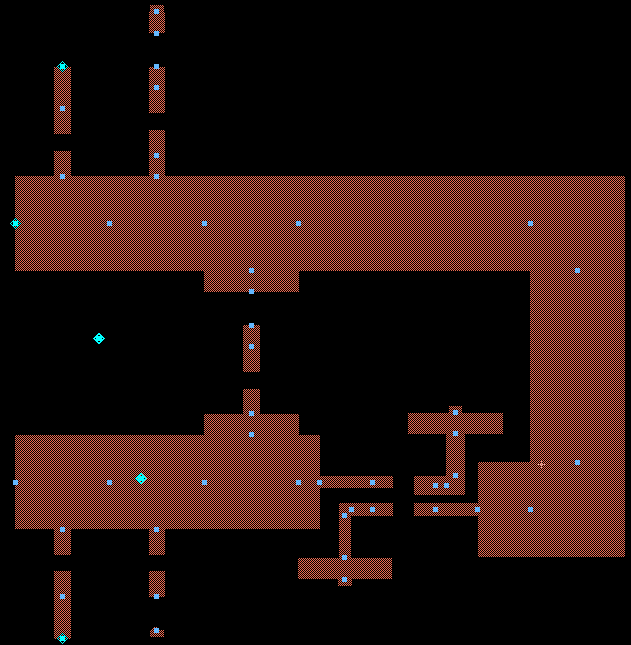
\includegraphics[width=2.5in]{LNApics/LNAlayout.png}
\caption{SAV-541+ transistor layout.}
\label{fig:lnaLayout}
\end{figure}

\begin{thebibliography}{1}
\bibitem{payne}
K. Payne, "Practical RF Amplifier Design Using the Available Gain Procedure and the Advanced Design System EM/Circuit Co-Simulation Capability," Agilent Technologies (5990-3356EN), 2008.
\bibitem{sav541datasheet}
Minicircuit SAV-541+ Datasheet
\end{thebibliography}
\end{document}